\clearpage \newpage 
\section{Diagrammer af kredsløb i systemet} \label{bilag:diagrammer}
\begin{figure}[h!]
	\centering
	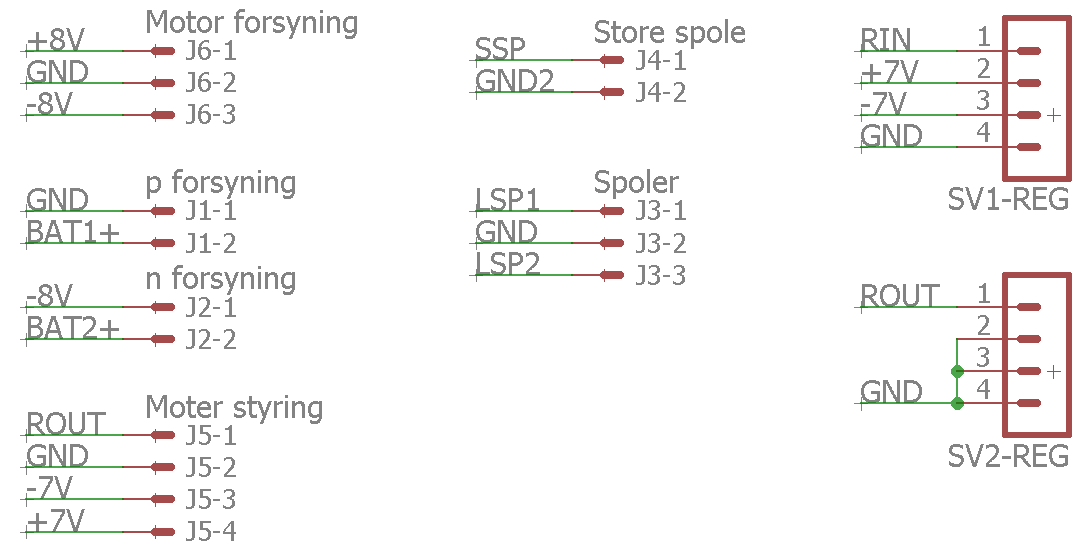
\includegraphics[width=.6\textwidth]{billeder/sch3_connectors.png}
	\caption{Diagram af connectors}
	\label{dig:sch3_connector}
\end{figure}
\begin{figure}[h!]
	\centering
	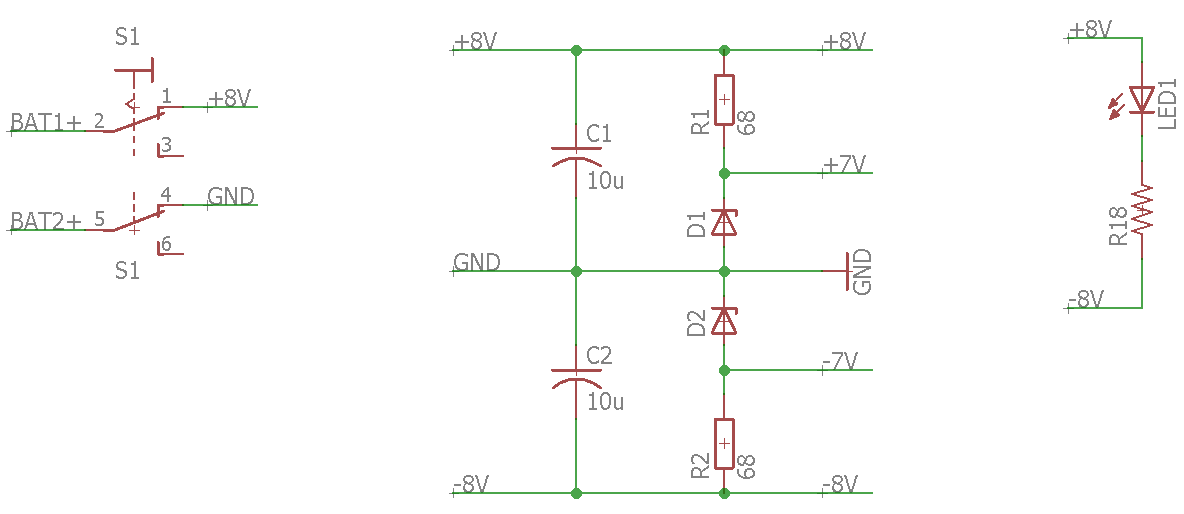
\includegraphics[width=.8\textwidth]{billeder/sch2_power_sw.png}
	\caption{Diagram af kontakt, power-LED, og shunt-regulator}
	\label{dig:power_sw}
\end{figure}
\begin{figure}[h!]
	\centering
	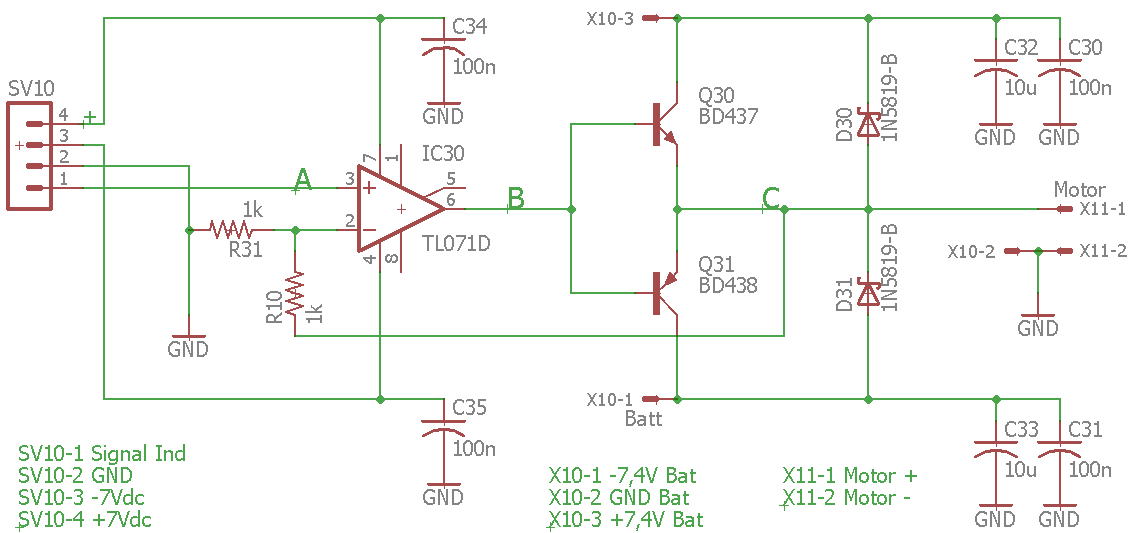
\includegraphics[width=1\textwidth]{billeder/motor_cont_schematic.png}
	\caption{Diagram af motor styringen}
	\label{dig:motor_diagram}
\end{figure}
\begin{figure}[h!]
	\centering
	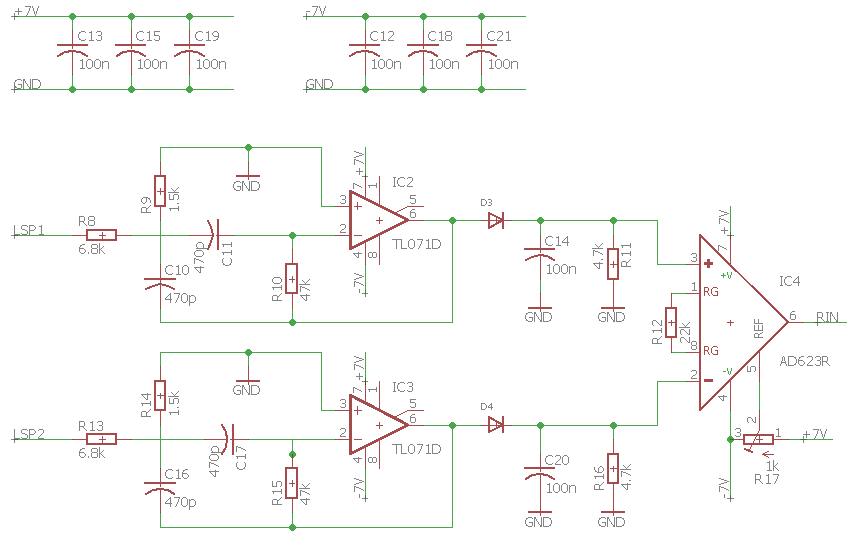
\includegraphics[width=1\textwidth]{billeder/sch1_signal1.png}
	\caption{Diagram af kredsløb til signalbehandling.}
	\label{dig:sch1_signal1}
\end{figure}
\begin{figure}[h!]
	\centering
	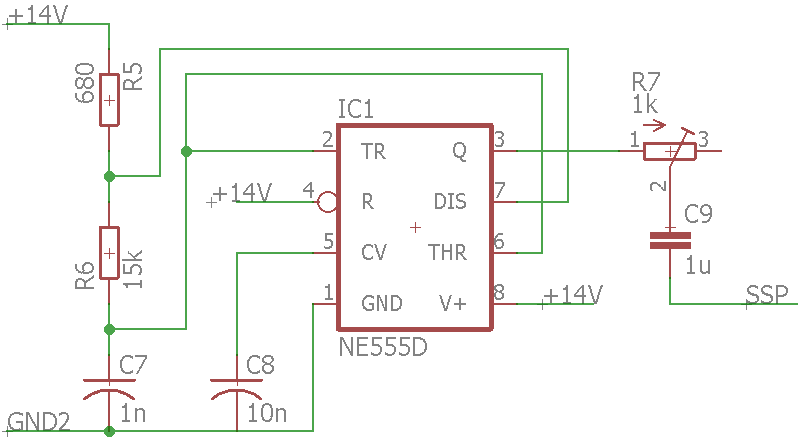
\includegraphics[width=.5\textwidth]{billeder/generator.png}
	\caption{Diagram af frekvensgenerator.}
	\label{dig:generator}
\end{figure}
\begin{figure}[h!]
	\centering
	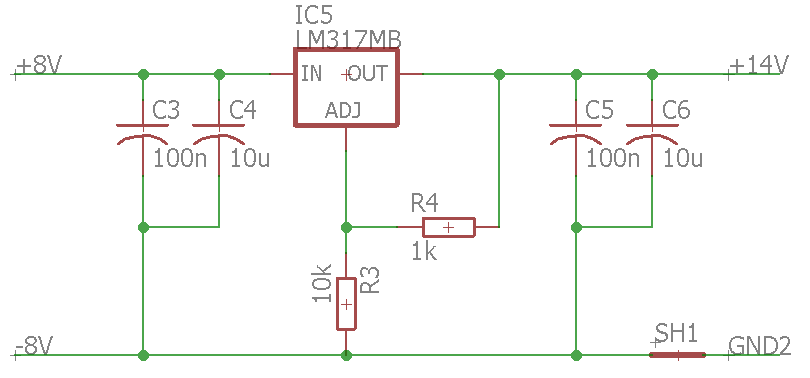
\includegraphics[width=.6\textwidth]{billeder/voltage_regulator.png}
	\caption{Diagram af spændings regulator}
	\label{dig:voltage_regulator}
\end{figure}
\begin{figure}[h!]
	\centering
	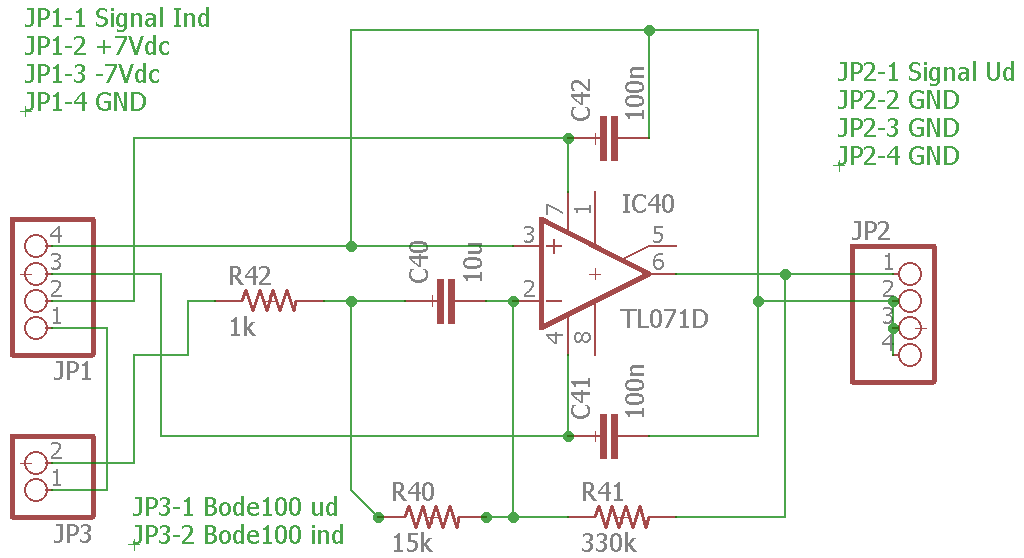
\includegraphics[width=.8\textwidth]{billeder/pd_schematic.png}
	\caption{Diagram af PD-regulator.}
	\label{dig:pd_schematic}
\end{figure}
\FloatBlock



